%%%%%%%%%%%%%%%%%%%%%%%%%%%%%%%%%%%%%%%%%%%%%%%%%%%%%%%%%%%%%%%%%%%
%                                                                 %
%                            CHAPTER                              %
%                                                                 %
%%%%%%%%%%%%%%%%%%%%%%%%%%%%%%%%%%%%%%%%%%%%%%%%%%%%%%%%%%%%%%%%%%%

\chapter{Literature study}
In this chapter we will take a quick look at how convolutional neural networks (CNN) function, layer by layer. We will also learn how secure multiparty computation (MPC) in general is possible. Finaly, we will discuss the related work on combining these two subjects so far.

\section{Convolutional neural network}
Convolution neural networks (CNN) is a special type of neural network used for images. The spatial properties of the pixels in the image are used during the evaluation of the input, meaning the neighbouring pixels of a central pixel impact the output to the next layer of that central pixel while pixels further away do not.
CNNs are made of multiple layers. Typically, as you move further from the input layer to the output layer the dimensionality reduces, we can say the input gets mapped on a desired output manifold. Inputs that we classify as similar are supposed to be in the same region in the output manifold. Neural networks go through two phases: training and interference. A neural network needs to be trained in order to achieve good results. After the training the network will try to predict things based on the inputted data, in this phase the parameters of the network do not chance.

\subsection{Convolution layer}
In this layer a discrete convolution of a kernel $K$ shifting over an image $I$ is performed, as shown in equation \ref{eq:1}. The kernel has parameters also called weights, so that certain features get extracted from the input.
\begin{equation} \label{eq:1}
  (I*K)[m,n]=\sum_j\sum_k I[m-j,n-k]K[j,k]
\end{equation}
The output of this layer is a convolved feature map. The parameters of the kernel are usually floating-point numbers and can be positive or negative.

\subsection{Activation function}
Since these convolutions are simple lineair operations and most image classification tasks require non-lineair classifiers, non-lineairity needs to be added to the neural network. This is achieved through adding a non-linear activation function after a convolution or fully connected layer. The most popular activation function is the rectified linear unit (ReLU) as seen in equation \ref{eq:2} and figure \ref{fig:relu}.
\begin{equation} \label{eq:2}
  f(x)=max(0,x)
\end{equation}

\begin{figure}[H]
  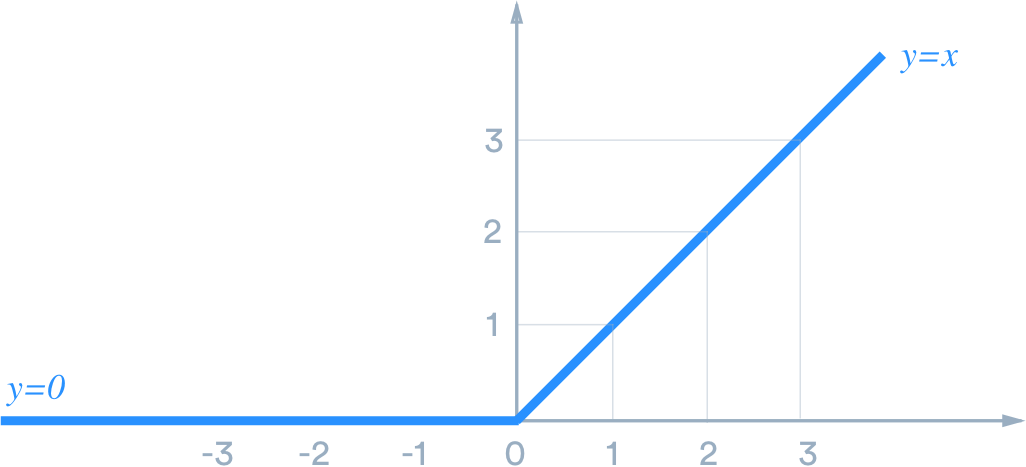
\includegraphics[width=\linewidth]{plots/relu.png}
  \caption{ReLu activation function}
  \label{fig:relu}
\end{figure}

\subsection{Pooling layer}
The dimensionality reduction we talked about in the beginning of this chapter happens in the pooling layer. A kernel is shifted over the image. In the case of max-pooling the kernel selects the maximum value of the portion of the image it covers, to create the new dimensionality reduced image. A portion of the image value is theoretically lost, but because we only retain the maximum value in the window we sort of extract a feature from the input matrix. An example of this process can be seen in figure \ref{fig:pooling}
\begin{figure}[H]
  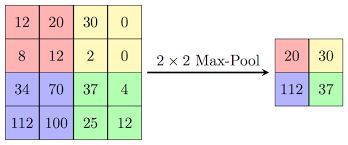
\includegraphics[width=\linewidth]{fig/maxpool.png}
  \caption{Example of $2\times2$ max-pooling}
  \label{fig:pooling}
\end{figure}

\subsection{Fully connected layer}
The fully connected layer is a multilayer perceptron that discriminates different object classes and identifies identical ones. All elements in vector $h_{i-1}^{out}$ have their own bias $B_i$ and weight $W_i$ so that $h_i^{in}$ can be calculated for each layer $i$ according to equation \ref{eq:3}.
\begin{equation} \label{eq:3}
  h_i^{in} = h_{i-1}^{out} \cdot W_i + B_i
\end{equation}

The fully connected layers usually comes after the last convolution layer. The output of a convolution layer is a tensor, this means that the output needs to be flattened to a one-dimensional array. The last layer of the fully connected layers is called the output layer. This output layer determines the classification.

\begin{figure}[H]
  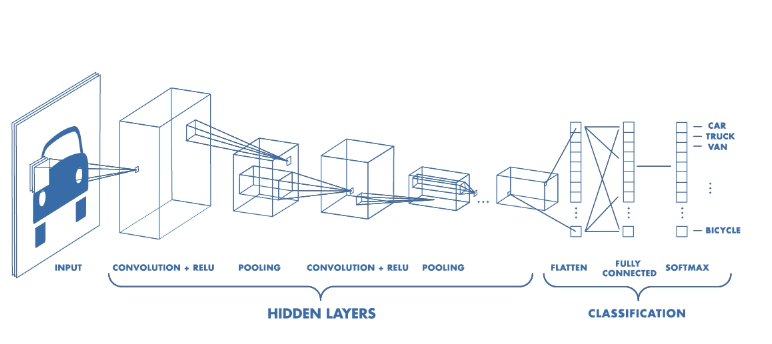
\includegraphics[width=\linewidth]{fig/cnn.png}
  \caption{Overview of CNN}
  \label{fig:cnn}
\end{figure}

When all these layers are connected to eachother, as you can see in figure \ref{fig:cnn}, we speak of a model with a CNN architecture.

\subsection{Face matching}
Face matching is an algorithm that tries to match two faces of the same person. Face matching can be performed with convolutional neural networks an image gets fed to the network and produces an output vector depending on what face was in the image. \cite{koch2015siamese} showed that a siamese neural network makes it possible to not only recognise new data (unseen during the training) but to also recognise entirely new classes. In the case of face matching each person's face is a class. With siamese neural networks it is thus possible to recognise faces of persons which the network didn't see during training.

A siamese neural network consists of two CNN's. These CNN's are identical. A siamese neural network has to be fed two images, it then produces two output vectors. When these two images have faces that are similar the euclidean distance between the two output vectors will be small. When the two faces on the images are dissimilar, the euclidean distance between the two vectors is large. Thus to determine if two images are of the same person, we calculate the euclidean distance (equation \ref{eq:distance}) between the two output vectors, if the distance lies under a certain threshold we accept that the two faces belong to the same person. If one output vector of the two images is stored in a database, an application can use this algorithm to allow for biometric authentication. This output vector is also referred to as the embedding of the face or a point on a manifold. A general overview of a siamese neural network architecture can be found in figure \ref{fig:siamese}.

\begin{equation} \label{eq:distance}
  d(p,q) = \sqrt{\sum_{i=1}^{n}(q_{i}-p_{i})^{2}}
\end{equation}

\begin{figure}[H]
  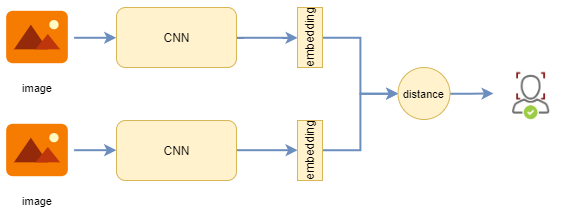
\includegraphics[width=\linewidth]{fig/siamese.png}
  \caption{Overview of siamese neural network}
  \label{fig:siamese}
\end{figure}

\section{Secure multiparty computation}
Secure multiparty coputation is a protocol that is used between $n$ number of parties $P$. Each of these parties has private data also called a secret $S$. With MPC it is possible for these parties to compute a public\footnote{public or global means known to all parties, while private or local means known only by the corresponding party} function $f$ on the secrets. Such that a party $P_i \in P$ only knows his secret $s_i \in S$ and the public securely computed output $f(s_0,s_2,s_{n-1})$ after the protocol has succesfully finished.
\newline
A classic application is Yao's Millionaires' problem \cite{yao1982protocols} in wich two millionaires wish to know who is richer, there is catch however. Instead of making their balances publicly known. They wish to keep their balances a secret. In this case the number of parties $n$ is 2 the secrets $s_0$ and $s_1$ are their balances. The public function $f(s_0,s_1)=1$ if $s_0<s_1$ and $0$ otherwise.

We categorize 2 types of parties based on their willingness to deviate from the correct predefined protocol.
\begin{itemize}
  \item \textbf{Honest parties:} Parties do not wish to know other parties secrets and will never reveal the secret.
  \item \textbf{Honest but curious parties (passive):} Parties wish to know other parties secrets but will not deviate from the protocol at any time. Also called semi-honest parties.
  \item \textbf{Malicious parties (active):} Parties wish to know other parties secrets and wish to change output of computation to favourable result. Parties will deviate from the protocol to cheat and change the outcome at any time.
\end{itemize}
In practice the whole set of parties will exist of subsets of these different types of parties. Ideally every party is honest, but this is rather a naive way of thinking.


If the two millionaires are honest but curious parties, they will not deviate from the protocol and they will computer the correct output as a result they will know who is the richer millionair but they won't know how much money the other one has. In the other case one of the two millionaires is corrupt and acts maliciously, the honest millionair will follow protocol while the dishonest millionair will deviate from the protocol to change the result in his favour. In the event that the dishonest millionair is poorer he will change the outcome thus appearing richer.
From now on, we assume the set of parties are a mix of honest and semi-honest parties, unless specified otherwise. We also assume the communication between the different parties to be secure.

The efficiency of an MPC protocol is defined by three metrics:
\begin{itemize}
  \item \textbf{round complexity:} The amount of rounds needed in the protocol. In one round each party can read all messages sent to the party in the previous round aswell as perform an arbitrary amount of local computation and finally send messages to all other parties.
  \item \textbf{communication complexity:} The amount of communication between all parties (measured in bits).
  \item \textbf{computational complexity:} The number of primitive operations performed by all parties.
\end{itemize}
In general, the computational complexity is very low while the communication complexity dominates the protocols total complexity. Thus an estimate of the overall complexity can be measured by combining the round and communication complexity. This means the efficiency of MPC protocols  is heavily based on the network's latency rather than the network's throughput.

\subsection{Secret sharing}
In order to do secure computing, the parties need to split their secret into secret shares. A secret sharing method can be used by the secret holder to split a secret into a number of shares. Combining these shares will reveal the secret, while individual shares alone will leak nothing about the secret. In a $(t,n)$ threshold secret sharing sheme parties must combine atleast $t$ shares of the total $n$ shares, to obtain the secret. We can now set a threshold $t$ high enough, denying the secret to small curious parties and allowing to reveal the secret when a majority ($\geq t$) consensus is reached. Shamir's secret sharing scheme \cite{shamir1979share} is based on polynomial interpolation and the essential idea is that it takes atleast $t$ points in order to define a polynomial $p(x)$ of degree $t-1$. Given a set of $t$ points in a 2-dimensional carthesian system  $(x_1, y_1), (x_2, y_2), ..., (x_t,y_t)$, there exists only one polynomial of degree $t-1$. This can be proven and the mathematical construction of a polynomial $p(x)$ of degree $t-1$ based on a set of $t$ points can be calculated using Lagrange's interpolation formula \ref{eq:5}.

\begin{equation} \label{eq:5}
\begin{aligned}
  p(x)= \sum_{i=1}^{t}y_{i}\delta_{i}(x)\text{\space\space\space\space with\space\space }\delta_{i}(x)=\prod_{1\leq j<t; i\neq j} \frac{x-x_i}{x_j-x_i}
\end{aligned}
\end{equation}

With this in mind, a secret dealer can now share his secret $s$ to $n$ parties by choosing a random $t-1$ degree polynomial $p(x)=a_{0} + a_{1}x + ... + a_{t-1}x^{t-1}$ in which $a_{0}$ is the secret or the number representation of the secret if the secret is not a number. The dealer now calculates $n$ points on the polynomial starting from $x=1$, because the secret is located at $x=0$. Each party $P_i \in {P_1, P_2, ..., P_n}$ is given a different single point $(x_i,y_i)$, at this stage the secret is shared. The convention for the notation of a shared secret is $[s]$. We can say a party $P_i$ is holding a share in the form of a point $(x_i,y_i)$ or shortened $[s]_i$.


\begin{figure}
  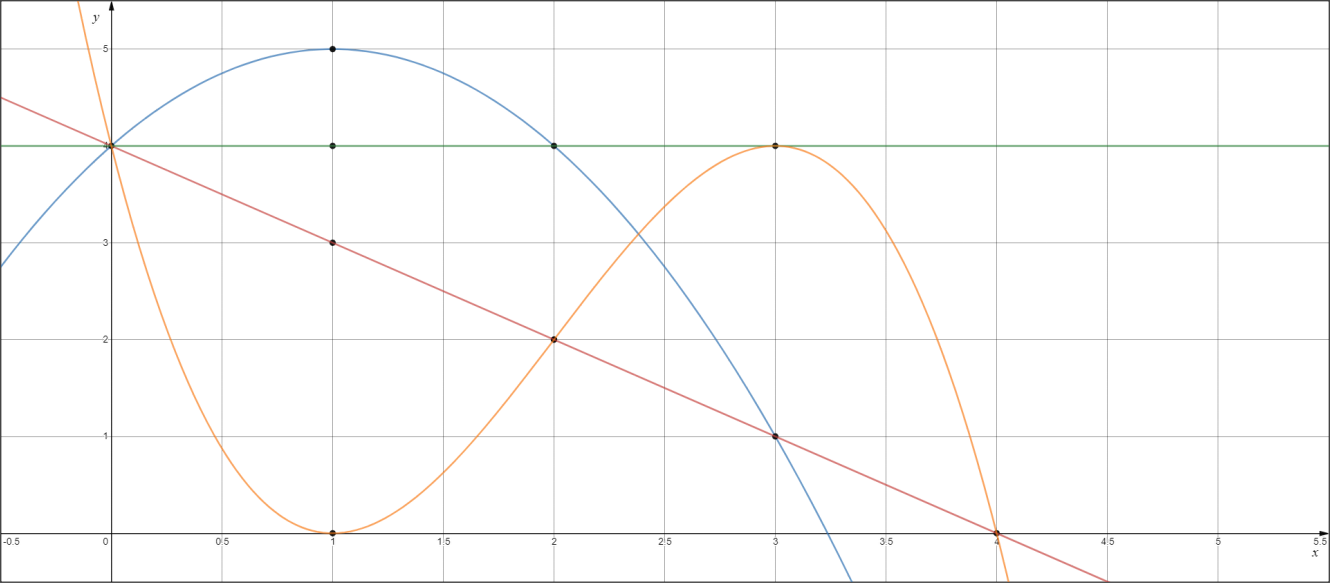
\includegraphics[width=\linewidth]{plots/secretsharing_big.png}
  \caption{Shares for different $t$ with secret $s=4$}
  \label{fig:secretsharing}
\end{figure}

To recombine the secret, the parties simply broadcast or send their shares to a central entity, if more than $t$ shares are known, it suffices to calculate the Lagrange polynomial $p(x)$ and $s=p(0)$. In the case of not having enough shares, the Lagrange polynomial containing the secret becomes impossible to calculate since every polynomial is equally likely, thus revealing absolutely nothing about the secret.

Note that all arithmetic in this section can be done over some finite field $\mathbb{F}_q$ to speed up the algorithms.

A Generalisation of this $(t,n)$-Shamir secret sharing scheme from thesis \cite{de2012design} as follows (Protocol 2.1 and Protocol 2.2):
\begin{enumerate}
  \item \textbf{Share Generation:} To share $s \in \mathbb{F}_q$, the dealer generates random $a_1, ..., a_t \in \mathbb{F}_q$ and puts $p(x) = s + a_1x + ... + a_tx_t$. Then the dealer computes $[s]_i = p(i)$.
  \item \textbf{Share Distribution:} For each $i \in {1, ..., n}$, the dealer sends $[s]_i$ to party $P_i$.
  \item \textbf{Secret Reconstruction:} Let $D \subset {1, ..., n}$ be a set of size $t + 1$. Each party $P_i$ for $i \in D$ sends his share $[s]_i$ to all parties. Then, each party reconstructs the secret via Lagrange interpolation.
\end{enumerate}
In figure \ref{fig:secretsharing} a visualisation of this scheme shows us that in order to get the secret value, $s=4$ in this case, we need to know atleast $t+1$ points for a given $t$. The trivial case where $t=0$ (green line) is simple to understand. The secret is simply the y-value of the given point. Of course this is a rather useless approach to secret sharing since you are giving away the cleartext secret. The full potential of secret sharing becomes true for cases where $t>0$. Two points are needed for a first order polynomial (red line), three points for a second order polynomial and so on.

It's important to make sure the parties are distributed and to try minimizing the incentive to collude. Distribution is needed to lower the risk of having a malicious party taking over control of the network, this can be done by splitting the parties up to many small stakeholders instead of a couple centralized stakeholders. We can only totally avoid collusion if the secret holder partakes to the MPC.

\subsection{Operations}
A neural network can be seen as an enormous function with millions of coefficients. Lucky for us the function can be broken up into 3 different operations: addition and multiplication in fully connected and convolution layers and a relational operator for max pooling and ReLU activation function. We will now show how to securely compute each of these basic operations.

\subsubsection{Arithmetic operators}
Addition, subtraction, division and multiplication all fall under the arithmetic operators. In this section we will take a look at how these operations can be performed in MPC.
\paragraph{linear protocols:}
Since Shamir's secrete sharing scheme is a linear sharing scheme, each party $Pi$ can locally compute any linear combination of a public or secret value with their secret share $[s]_i$. This gives us following operations:
\begin{itemize}
  \item \textbf{Addition of secret and public value ($[c] \gets [a] + \beta$):} Each party $P_i$ locally adds the public value $\beta \in \mathbb{F}_q$ to it's share $[a]_i$, resulting in the new share $[c]_i = [a]_i + \beta$. Since all parties add the same $\beta$, this value is a constant.
  \item \textbf{Multiplication of secret and public value ($[c] \gets [a] \cdot \beta$):} Each party $P_i$ locally multiplies the public (constant) value $\beta \in \mathbb{F}_q$ with it's share $[a]_i$, resulting in the new share $[c]_i = [a]_i \cdot \beta$.
  \item \textbf{Addition of multiple secrets ($[c] \gets [a] \cdot [b]$):} Each party $P_i$ locally adds it's secret shares $[a]_i$ and $[b]_i$, resulting in the new share $[c]_i = [a]_i + [b]_i$.
\end{itemize}

The last operation is visually demonstrated in figure \ref{fig:addsecrets}. In this example secret $a=1$ (green) and secret $b=3$ (red). After each party $P_i$ locally computes the addition of $[a]_i$ and $[b]_i$ and stores it as a new share $[c]_i$. After broadcasting the new, computated share $[c]$. They can recombine the shares via Lagrange interpolation to get the polynomial of the combined shares $[c]$ and more importantly the output of the addition of the two secrets $a$ and $b$. This happens all with zero knowledge about $a$ or $b$. All of the computations are done locally and no communication other than the inital share distribution and the share reconstruction is needed.

\begin{figure}
  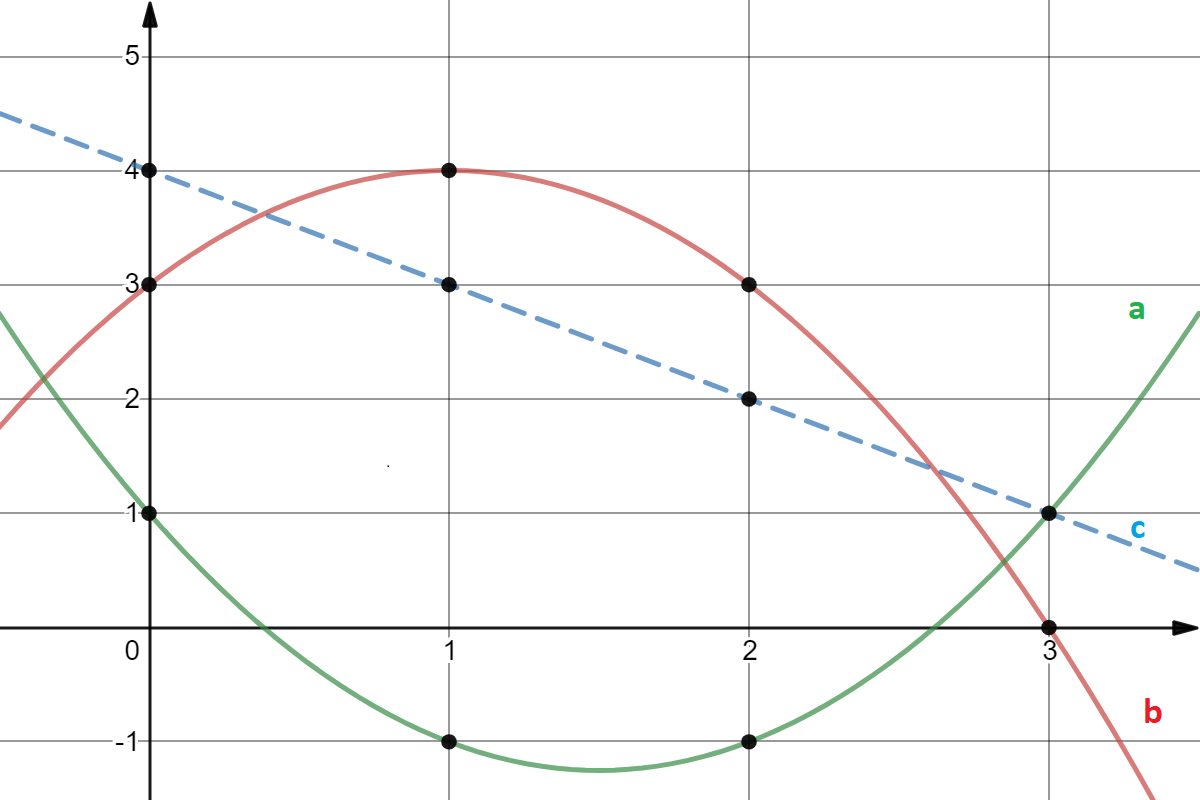
\includegraphics[width=\linewidth]{plots/addsecrets.png}
  \caption{Adding two secrets for $n=3$ parties}
  \label{fig:addsecrets}
\end{figure}

The inverse operations (subtraction and division) are possible too, and the protocol is the same.

\paragraph{Multiplication protocol:}
Multiplication of two secret values is more challenging since it isn't a linear operation. Their are multiple methods to perform secret multiplication, the method described by \cite{ben1988completeness} also called the BGW protocol (initials of the authors) has to solve two problems along the way of computing $c = a \cdot b$.

Assume $a$ and $b$ are respectively encoded by $f(x)$ and $g(x)$ and $n \geq 2t + 1$. The free coefficient of $h(x) = f(x) \cdot g(x)$ is simply $h(0) = f(0) \cdot g(0)$, this means a simple multiplication of the polynomials would be sufficient to compute the multiplication of the secrets. There is however a major problem, multiplication of two polynomials of degree $t$ yields a polynomial of degree $2t$.

While this poses no problem with interpolating $h(x)$ from it's shares $[c]$ since $n \geq 2t + 1$, further multiplications will continue to raise the degree to a level where $t>n$ making it impossible to interpolate the resulting polynomial $h(x)$. The second problem is harder to spot.
The polynomial $h(x)$ as a result of the multiplication of polynomials $f(x)$ and $g(x)$ is reducible (since it's a multiplication).

In other words $f(x)$ and $g(x)$ are uniformly random polynomials of degree $t$, but $h(x)$ as a multiplication of two random polynomials is not irreducible, therefore $h(x)$ is not uniformly random. To make sure the resulting polynomial stays of degree $t$ and is uniformly random, the parties run a protocol to generate a random polynomial of degree $2t$.

This protocol works as follows. Each party $P_i$ randomly selects a private polynomial $q_i(x)$ with secret $q_i(0) = 0$ of degree $2t$ and distributes it's shares among the parties. Each party $P_i$ now has $n$ random shares $[q]_i^k$ (with $k: 1 \rightarrow n$). After each party adds all it's random shares they hold a secret, truly random polynomial $q(x)$ with a zero as free coefficient $q(0) = 0$.
Each party $P_i$ now computes the multiplication of the two secret values $[a]$ and $[b]$ and instead of using $[c]$ encoded as $h(x)$ we can add the random polynomial to the result, thus randomizing the coefficients and making the polynomial uniformly random. This will not mess up the result as now $a \cdot b$  is $(f(0) \cdot g(0)) + q(0)$ and $q(0)$ equals zero. This step is also called the randomization step.


The parties now run a protocol to reduce the degree of $h(x)$ to $t$. This protocol can be computed locally (no communication is required) by multiplying the shares of the polynomial $h(x)$ to a specific, matrix of constants. This will truncate the result $h(x)$ of degree $2t$ to a polynomial of degree $t$. Proof for this degree reduction step can be found in the study by \cite{asharov2017full}.


After these two steps, the parties hold $c =a \cdot b$ encoded by $h(x)$ of degree $t$ with coefficients uniformly distributed. They can now recombine their shares to find the polynomial $h(x)$ and the product of $a$ and $b$, $h(0)$. The whole multiplication protocol requires only one additional round of communication, this happens during the distrubition of the shares of the random polynomials $q(x)_i$ in the randomization step. Note that since we conditioned the protocol to work in cases where $n \geq 2t + 1$, a majority of honest parties is needed. Opposed to the linear protocols explained earlier, where only one party needed to be honest.


A large proportion of the neural network is ready to be transformed with these secure arithmetic operators, namely the convolution layer and the fully connected layer.

\subsubsection{Relational operators}
In this section we will focus on comparison between secrets. There are two important protocols in secure comparison, equality testing and greater-than testing.

\paragraph{Equality testing:}
Suppose we have two shared secrets $[a]$ and $[b]$ and the parties want to know if $a = b$, without knowing $a$ or $b$.
The easy way, would be to just securely compute and reveal $c = a - b$. This would however reveal secret $b$ if $a$ was to be revealed, since $b = a - c$. To make sure the the output of the subtraction is irreducible and uniformly random \cite{franklin1996joint} came up with an idea to let the parties generate a random shared non-zero secret $[r]$.
Then compute and reveal $c = (a - b) \cdot r$. Since $r \neq 0$, if $c = 0$, $a$ must be equal to $b$. If $c \neq 0$, $a$ and $b$ are not equal. If we want to compare a secret with a public value $\beta$, we just take $a$ as the secret and use a $\beta$ instead of $[b]$ in the protocol. In this case the naive method $c = (a - \beta)$ would just give away the secret value even if $a \neq \beta$, so it's absolutely required to use a random multiplier $r$ to hide the reversible operation.

The generation of a random shared non-zero secret $[r]$ appears to be very similar to the generation of the random share in the randomization step of the multiplication protocol but there is one difference, in this case the secret value must be different than zero (invertible), while in the multiplication protocol the random share needed to be equal to zero. The idea is to generate two shared random secrets $[x]$ and $[y]$. Then the parties compute the product of the two secrets $z = x \cdot y$ and reveal $z$. If $z \neq 0$, both random secrets $x$ and $y$ are non-zero, thus applicable in the equality testing protocol. If $z = 0$ repeat the random share generation protocol with different random shared secrets and retry the multiplication with these new shares.

\paragraph{Greater-than testing:}
Often we want to know more about two secrets than just equal or different. We want a protocol comparing two secrets $a$ and $b$ that returns a boolean for $a>b$. There exists multiple different protocols for greater-than comparisons. The one we use in our implementation is published in \cite{erkin2009privacy}. This protocol compares the two secrets on bit-level.

\subsection{Number representation}
When a CNN gets computed on cleartext data almost all parameters of the CNN are floating-points, it is thus important that these numbers can be transformed to representations suitable for MPC.

Floating-points can be implemented in MPC. But they usually come with a high complexity cost for addition aswell as multiplication and comparison tests. The advantage of floats over other number representations like scaled integers and fixed-point numbers is that the the maximal rounding error scales with the magnitude of the number. Unlike floats fixed-points have a rounding error of a fixed size. \cite{campmans2018optimizing} studied the use of fixed-point numbers as an alternative for floating-point numbers in MPC protocols. He states that with fixed-point numbers no comparison needs to be done during multiplication of two secrets. While the costly comparison is needed when multiplicating two secret floating-point numbers.

A fixed point data type is essentialy an integer that is scaled by a chosen factor. Let's say our numbers in the MPC protocol never go out of the bounds $[-500,500]$ and we want a precision of 2 fractional digits. Then we can use the integers bounded by $[-50000,50000]$ to perform all arithmetic. The arithmetic operations will be the same as when we use integers. But we will actually be computing arithmetic operations on fixed-point numbers. This allows for an efficient approach to floating-point numbers while minimizing rounding errors. Of course we need to make sure that the operations don't overflow and that precision loss is small.

\section{Overview}
We now have seen the miscellaneous protocols MPC has to offer. From now on we will treat the seen MPC protocols like black boxes that accept inputs in the form of secret shares and compute outputs in the form of secret shares. As long as the parties do not collude to find the secret, the protocol is secure.\\
Overview of protocols:
\begin{itemize}
  \item Secure addition of two secrets or a secret and a public value ($F_{add}$).
  \item Secure multiplication of secret and public value ($F_{mul}^{constant}$).
  \item Secure multiplication of two secrets ($F_{mul}$).
  \item Equality testing of two secrets or a secret and public value ($F_{eq}$).
  \item Greater-than testing of two secrets ($F_{gt}$).
\end{itemize}

This set of protocols can be used to transform any basic CNN to a secure one.

In figure \ref{fig:workflow} a high-level workflow of secure face recognition is shown. The MPC protocol works for three parties \footnote{This is the smallest amount of parties needed in order to do secure multiplication ($F_{mul}$).}, who each have their own computing instance connected to the MPC network and the client. The workflow commences by acquiring an image of the clients face, this can be done by taking a photograph with the front-facing camera of the clients smartphone. The client then performs secret sharing on the image \footnote{Secret sharing is performed for each pixel of the image.} and sends the shared secret to the participating parties. The parties receive their shares and jointly compute the output of the face recognition model on the given shared image of the face. The face recognition model can be public or secret. In the case of a secret model, the secret shares of the weights and biases need to be sent to the participating parties aswell. Note that this only has to be done once, during initialisation. After the computation is finished, the parties send their resulting secret shares to the client. The client interpolates the shares to find the secret values determining if her face matches or not.


This protocol ensures that the client is the only one having knowledge about the cleartext of the image and the output of the face recognition algortihm. This protocol also offers an obfuscation of the model's parameters, the parties and the client have no knowledge about the parameters if the owner of the model uses secret sharing to send the parameters to the parties.

\begin{figure}
  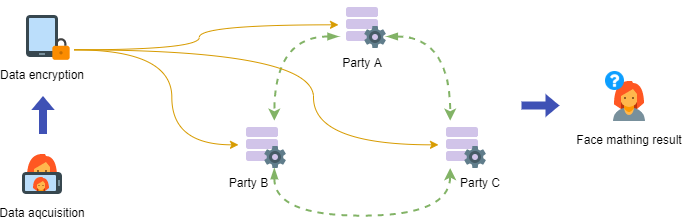
\includegraphics[width=\linewidth]{fig/workflow.png}
  \caption{Workflow of secure face matching}
  \label{fig:workflow}
\end{figure}

\section{Related work}
\cite{erkin2009privacy} presented for the first time a privacy-preserving face recognition alogithm using MPC, this was before the rise of machine learning. Thus they were restricted to using eigenvalues of the faces described in \cite{turk1991face}. They show that their privacy-preserving face recognition algorithm is as reliable as the normal face recognition algorithm. Unfortunately, the computational cost for producing the eigenvalues of an image is way less than producing a result for a CNN.

\cite{mainali2019privacy} recently published the first framework for privacy-ehancing fall detection from a body-worn inertial measurement unit using traditional machine learning and MPC. The data they work with is time-series inertial measurements this has a significantly lower dimensionality than an image. Traditional machine learning classifiers require less computations than deep neural networks. The authors hint to secure video-based fall detection as a possibility future research and to which extent secure video-based fall detection can be performed real-time with high-dimensionality.

\cite{gilad2016cryptonets} discuss implementing CryptoNets, a fully homomorphic encryption (FHE) based approach for privacy-preserving optical character recognition task on the Modified National Institute of Standards and Technology (MNIST) database of handwritten digits. FHE is another approach to making machine learning privacy-preserving. But since we focus on MPC in this thesis, we refer the interested reader to the paper written by \cite{gentry2009fully}.

\cite{barni2006privacy} presented an algorithm that does privacy-preserving computation on a neural network using MPC. The data owner encrypts the input, via secret sharing, and sends the secret shares to the participating MPC parties. The parties compute the inner product of the weights of the layer and the data. The product gets sent back to the data owner. The data owner then adds non-linearity via an activation function on the outputs, this is done in cleartext since the data owner can decrypt the secret shares and is allowed to see is own data. The result then gets encrypted again and is sent to the MPC parties to compute the inner product in the second layer. This protocol is done for all the parties. In this algorithm the data owner communicates multiple times with the MPC parties. Some computation of the neural network is also done by the data owner. A strong cooperation between the parties and the data owner is thus needed.

\cite{campmans2018optimizing} worked on optimisation of existing MPC protocols for convolutional neural network operations. He also suggested using fixed-point numbers instead of floating-point, losing some accuracy for more efficiency. He also explored the use of discrete fourier transforms as an approach to costly convolutions in MPC. The convolutions are costly because they require lots of multiplications.

\cite{makri2019epic} proposed EPIC an efficient private immage classification system based on support vector machine (SVM) learning. They focus on efficiency by minimizing the load on the privacy-preserving part. Their experiments conclude that their is a tradeoff between efficiency and accuracy of the privacy-preserving image classification systems. They consider the deployment of a CNN with current MPC protocols in an active adversary MPC environment to be computationaly prohibitive. It should be noted that in our implementation, we assume the MPC environment to be made of passive adversaries.

\cite{taigman2014deepface} presented DeepFace, a face recognition algortihm trained on millions of images of Facebook users. It achieves a stunning 97.35\% on the Labeled Faces in the Wild (LFW) dataset, which is the classic benchmark dataset for face recognition, closing the gap to human-level perfomance. The authors made use of a siamese neural network. But this alogrithm is already outdated. Deep learning based networks use more layers than a regular neural network, \cite{wang2018deep} give an overview of the recently published alogrithms, most of them use a deep learning based architecture. Some of the alogrithms achieve an acurracy of around 99.8\% on the LFW dataset. This surpasses the ability of face recognition by humans. These neural networks often have millions if not billions of parameters. This means that the computational complexity is very high and it is unlikely that we will find a way to efficiently make this type of neural networks secure. Instead we will focus on slightly lighter neural networks with less layers and parameters.

\section{Conclusion}
It is theoretically possible to implement a privacy-preserving CNN that works just like a normal CNN on cleartext data. But in practice we expect some resistance based on the related work, the main problem is the complexity that arises when performing MPC protocols on high dimensional data like images. There is a tradeoff between precision and complexity. Our first steps shall be to implement a naive design of the MPC protocol for CNN's. Then we will try to improve the efficiency, by adding existing optimisation solutions, thus minimizing the time it takes to perform one face matching task. We will compare our results with other privacy-preserving techniques for CNN's.
